\documentclass[conference]{IEEEtran}
\usepackage[utf8]{inputenc}
\usepackage{amsmath,amssymb,amsfonts}
\usepackage{tikz}
\usepackage{color}
\usepackage{xcolor}
\usetikzlibrary{arrows.meta,patterns}
\usepackage{pict2e,color}
\usetikzlibrary{fit}
\usepackage{pgfplots}
\usepackage{color,soul}
\usetikzlibrary{positioning, arrows.meta,calc}
\usepackage[colorinlistoftodos,prependcaption,textsize=footnotesize]{todonotes}

\begin{document}

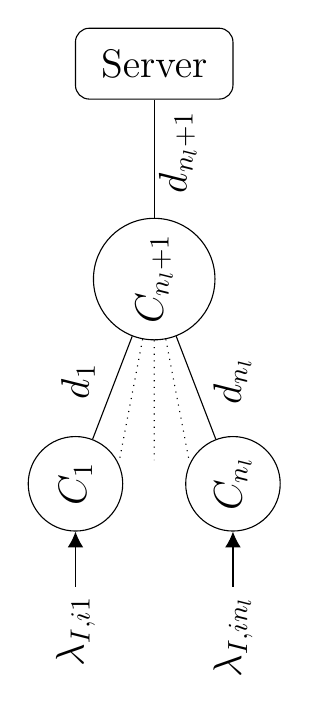
\begin{tikzpicture}[sibling distance=0.5cm, level distance = 2.6cm]
  \tikzset{
    parent/.style={draw, rectangle, rounded corners=5pt, minimum height=0.9cm, minimum width=2cm},
    child/.style={draw, circle, minimum size=1.2cm}
  }
  
  % Level 1
    \node [child,font=\Large] (parent1) {\rotatebox{90}{$C_{{n_l}+1}$}}
    child { node [child,font=\Large] (child1) {\rotatebox{90}{$C_1$}} } % Rotate the child node text
    child[dotted, shorten >= 0.3cm]
    child[dotted, shorten >= 0.3cm]
    child[dotted, shorten >= 0.3cm]
    child { node [child, font=\Large] (child2) {\rotatebox{90}{$C_{n_l}$}} }; % Rotate the child node text
    
  % Level 2
  \node [above=1.5cm of parent1, parent,font=\Large] (parent2) {Server};
  
  % Connect nodes
  \draw (parent1) -- (parent2);
  
  % Labels
  \node [below=0.7cm of child1,font=\Large] (word1) {\rotatebox{90}{$\lambda_{I,i1}$}};
  \node [below=0.7cm of child2,font=\Large] (word2) {\rotatebox{90}{$\lambda_{I,in_l}$}};
    
  % Word in the middle of vertical height
  \node [left=0.4cm of parent1, xshift=0.55cm, yshift=-1.3cm,font=\Large] (word3) {\rotatebox{90}{$d_1$}};
  \node [right=0.4cm of parent1,xshift=-0.55cm, yshift=-1.3cm,font=\Large] (word3) {\rotatebox{90}{$d_{n_l}$}};
  \node [above=0.09cm of parent1, yshift=0.1cm,xshift=0.3cm,font=\Large] (word3) {\rotatebox{90}{$d_{n_l+1}$}};

  % Arrows
  \draw[-{Latex[length=2mm,width=2mm]}, line width=0.5pt] (word1) -- (child1);
  \draw[-{Latex[length=2mm,width=2mm]}, line width=0.5pt] (word2) -- (child2);

\end{tikzpicture}

\end{document}